%Estado del arte y arquitectura propuesta
Previo al diseño de este sistema, es pertinente conocer el estado del arte de otros sistemas de adquisición de datos para física de partículas, con el fin de contrastar y rescatar las diferentes estrategias y tecnologías empleadas en la actualidad.

En las siguientes páginas se mencionan tres sistemas relacionados a esta temática, destacando ideas sobre el esquema general de adquisición de datos, tecnologías que se utilizan actualmente para construirlos y  métodos para adquirir y procesar las señales captadas.

\section{LabPet II}

	Como referencia para el diseño del sistema de adquisición, se han investigado detectores como los descritos en \cite{Basiladze2017Methods1} y \cite{Basiladze2017Methods2}, enfocados a detección de partículas en diferentes rubros y condiciones.
	
	Dentro de la variedad de detectores estudiados, LabPet II de Larissa Njejimana \cite{Njejimana2013DesignImaging} presenta una estructura clara e interesante. Este detector posee un DAQ distribuido en tres FPGAs, contando con etapas para recolectar, procesar y transmitir la información obtenida. Una primera etapa consiste en registrar tiempo, energía y posición de las partículas captadas; una segunda etapa ordena cronológicamente los eventos capturados, mientras que una tercera etapa agrupa detecciones coincidentes, calculando además la tasa de eventos aleatorios ocurridos. La figura \ref{fig:njejimana} ilustra este sistema.
	
	Si bien, dicho detector está diseñado para otro tipo de partículas (positrones), la naturaleza de las señales es muy similar, y por lo tanto la lógica para su adquisición y procesamiento es comparable. Aún así, la cantidad de señales que es capaz de manejar dicho dispositivo ronda las 64 señales por módulo, a tasas cercanas a los 2 millones de eventos por segundo, las que comparativamente sobrepasarían las necesidades del sistema a desarrollar en este proyecto de titulación. Por ejemplo, los rayos cósmicos cruzan el planeta tierra a aproximadamente 1 rayo cósmico por minuto en un área de $1cm^2$, muy por debajo de lo que se espera en LabPET II.
	
	Del sistema de adquisición para el detector anteriormente mencionado, se destaca la utilización de multiplexores, serializadores/deserializadores y memorias de almacenamiento temporal (\textit{buffer}). Dada la naturaleza y cantidad de eventos, se hace necesario serializar la información, ya que de otro modo sería necesario construir dispositivos con muchos puertos de entrada o incluir varios del mismo tipo. Además, debido a la frecuencia de eventos, se hace obligatoria la existencia de \textit{buffers} para el almacenamiento de la información, para así procesarlos y transmitirlos hacia etapas posteriores a tasas menores. Es destacable también la utilización de métodos para ordenar cronológicamente los eventos y la implementación del método TOT (Time-over-threshold) para el calculo de energía y datos temporales de pulsos analógicos. 
	
	\begin{figure}[h]
		\centering
		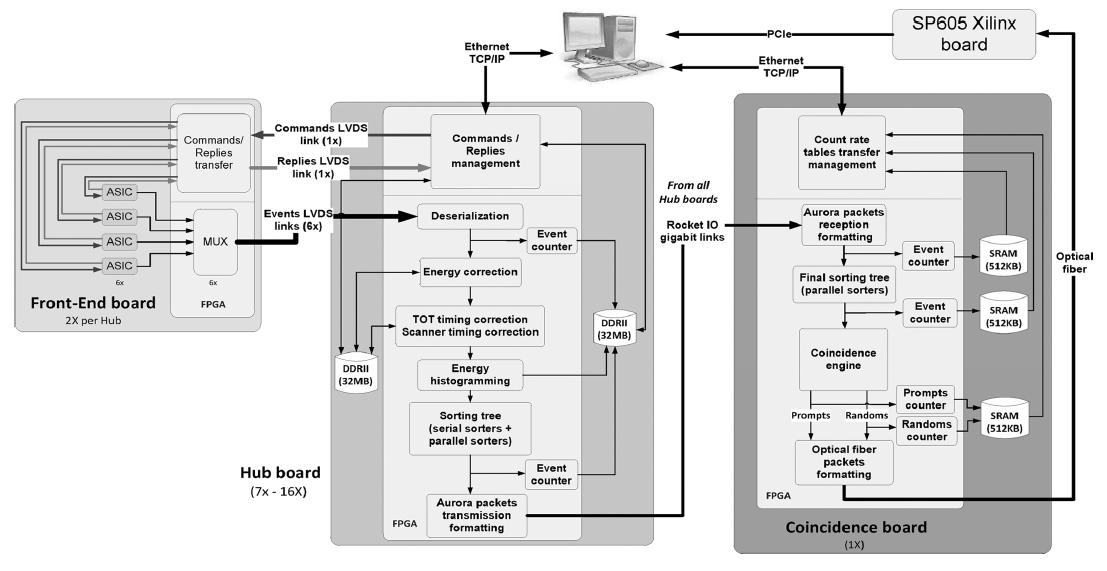
\includegraphics[scale=0.45]{njejimana.png}
		\caption{Diagrama de bloques del sistema de adquisición de datos para LabPET II \cite{Njejimana2013DesignImaging}}
		\label{fig:njejimana}
	\end{figure}
	
\newpage
\section{PET 4D}
	
	Otro sistema de referencia es el DAQ para un detector PET 4D \cite{Marcatili2011DevelopmentDetector}, similar al LabPET II. Este dispositivo permite capturar gran cantidad de señales provenientes de arreglos matriciales de fotomultiplicadores. Se caracteriza principalmente por poseer una tarjeta madre central en la cual es posible conectar hasta 18 tarjetas de adquisición. Cada una de estas últimas cuenta con 8 o hasta 32 canales para la adquisición de pulsos provenientes del detector, encargándose de capturar, procesar y enviar información a la placa madre.
	
	Las señales son capturadas por ASICs (\textit{Application Specific Integrated Circuits}), muestreadas por conversores análogo-digitales, procesadas por una FPGA y controladas por una FPGA principal (etiquetada como la placa madre). El procesamiento se encarga de calcular energía y datos temporales, mientras que el control final relaciona los eventos que hayan sido temporalmente coincidentes y calcula el tiempo de vuelvo de las partículas con apoyo de un conversor de tiempo a señal digital (TDC).
	
	Este sistema destaca por su modularidad, la cual permite escalamiento. En contraste con LabPET II, se sustituye la serialización de datos con la presencia de varias placas adquisidoras de datos, procesando la información antes de llegar a la FPGA principal. Cabe destacar que esta arquitectura está relacionada con la necesidad de encontrar múltiples eventos simultáneos en distintas ubicaciones físicas, requerimiento que no está presente en el sistema que se planea diseñar para este proyecto de titulación. La figura \ref{fig:marcatili} ilustra la arquitectura de este sistema.
	
	\begin{figure}[h]
		\centering
		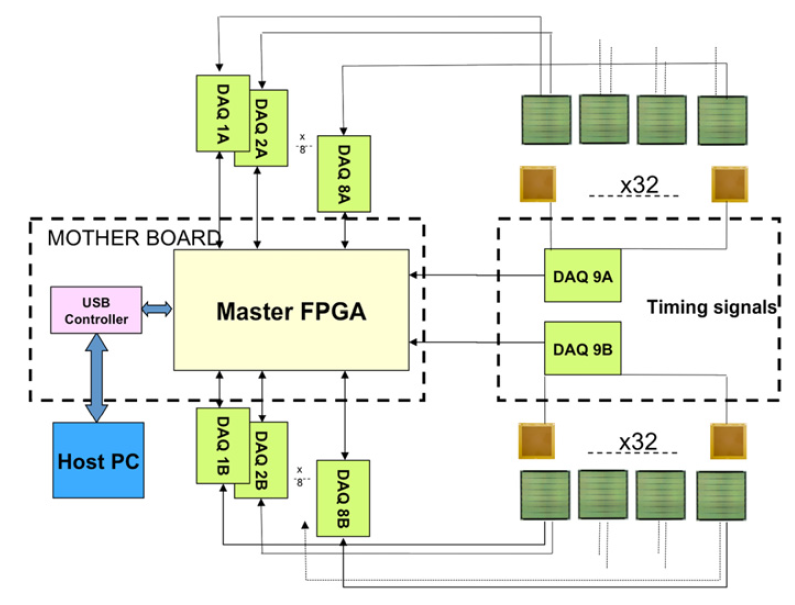
\includegraphics[scale=0.4]{marcatili.png}
		\caption{Diagrama de bloques del sistema de adquisición de datos para Detector PET 4D \cite{Marcatili2011DevelopmentDetector}}
		\label{fig:marcatili}
	\end{figure}
	
\newpage
\section{ATLAS}
	
	Finalmente, la referencia más importante corresponde a la del experimento ATLAS, donde se utiliza la misma tecnología de detectores y la misma interfaz de adquisición ASD (Amplificator-Shaper-Discriminator) en una de sus etapas, como se mencionada en \cite{Spieler2012ElectronicsAcquisition}.
	
	Este experimento intercepta grupos de partículas provenientes de haces de protones acelerados en el LHC (Large Hadron Collider) en CERN, produciendo colisiones entre sí cada $25\mu$s y generando cerca de 23 interacciones con el detector, que junto a otros factores implica cerca de $10^9$ eventos cada segundo \cite{Whiteson2016TheSystem}. La magnitud, tasa de aparición y nivel de energía de estos eventos son las principales razones de la complejidad tecnológica de este detector.
	
	Este detector posee dos etapas previas de selección de eventos, donde la primera etapa involucra detectores de muones y calorímetros, mientras que la segunda involucra algoritmos distribuidos en varios computadores. La figura \ref{fig:spieler} ilustra la interfaz para la captura de los pulsos generados por muones en los detectores (TGC).
	
	
	\begin{figure}[h]
		\centering
		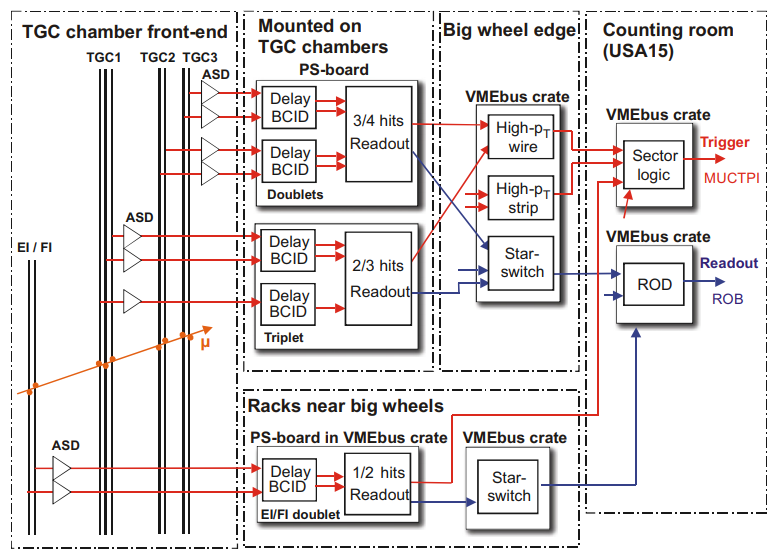
\includegraphics[scale=0.6]{spieler.png}
		\caption{Diagrama de la interfaz de lectura para detectores de muones \cite{Spieler2012ElectronicsAcquisition}. Los muones se representan con el símbolo $\mu$. Existen 3 capas de detectores, por lo tanto se observan 3 bloques que incluyen retardos, selección y captura de los pulsos.}
		\label{fig:spieler}
	\end{figure}
	
	\newpage
	Luego de generarse la primera señal de disparo, se da paso a la adquisición de datos en la tarjeta de lectura del detector (\textit{Readout System}), enviando paralelamente información sobre regiones de interés a analizar, con el fin de llevar a cabo la segunda etapa de selección de eventos mediante el disparo de alto nivel (\textit{High-Level Trigger}). Esta segunda señal de disparo utiliza software distribuido en cerca de 2000 computadores conectados a una red Ethernet y filtra eventos en función a muestras de datos pertenecientes a las regiones de interés calculadas por la etapa de disparo anterior, como se describe en \cite{Colombo2015Data-flowCase}. Finalmente, los eventos seleccionados son trasferidos y  almacenados en los bancos de datos del centro de investigación. La figura \ref{fig:colombo} ilustra las etapas mencionadas.
	
	\begin{figure}[h]
		\centering
		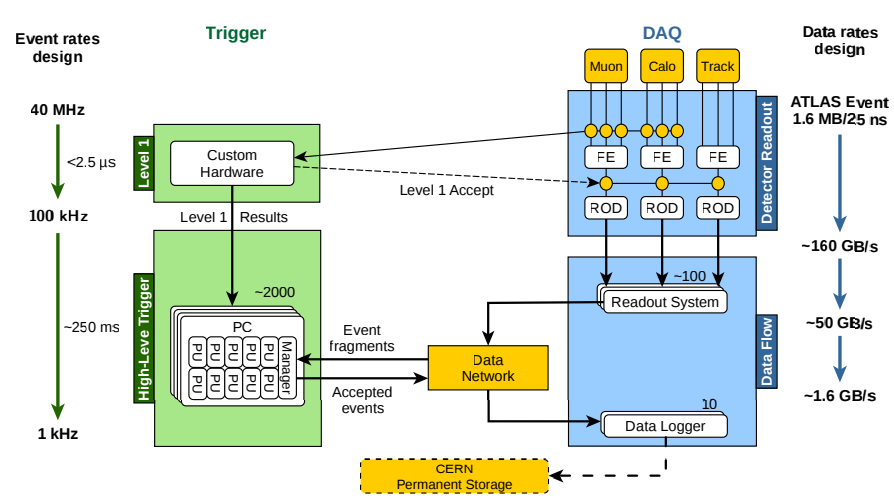
\includegraphics[scale=0.56]{colombo.png}
		\caption{Diagrama del sistema de disparo y adquisición de datos en el experimento ATLAS. \cite{Colombo2015Data-flowCase}}
		\label{fig:colombo}
	\end{figure}
	
	Entrando en detalle, según se indica en \cite{Whiteson2016TheSystem}, el verdadero sistema de adquisición de datos para este experimento es el software distribuido en red, capaz de discriminar, procesar y transferir los eventos seleccionados a los bancos de datos. El sistema lectura (\textit{Readout System}) en conjunto con el disparo de primer nivel solo serían un equivalente a una interfaz de captura muy sofisticada, más que las observadas en otros detectores, pero para el caso de esta memoria de titulación es comparable al sistema de adquisición que se desea diseñar.
	
	El sistema de lectura consiste en una tarjeta llamada ROBIN, compuesta de buffers, chips de comunicación, memoria flash, procesador y una FPGA, como se ilustra en la figura \ref{fig:whiteson}
	
	\begin{figure}[h]
		\centering
		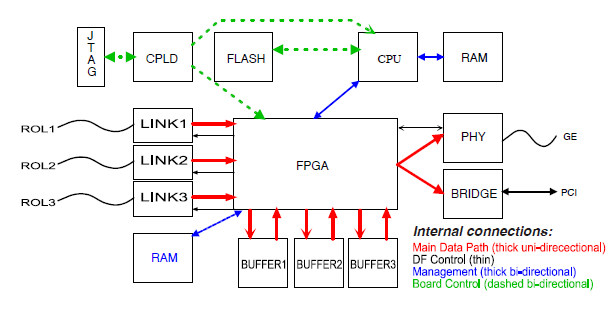
\includegraphics[scale=0.7]{whiteson.png}
		\caption{Diagrama de la tarjeta de lectura ROBIN en ATLAS \cite{Whiteson2016TheSystem}.}
		\label{fig:whiteson}
	\end{figure}
	
	La lógica descrita al interior de dicha FPGA se ilustra en la figura \ref{fig:whiteson2}. Se observa que su labor es principalmente controlar los buffers de datos, traspasar los eventos captados hacia la siguiente etapa y eliminar los datos descartados por la señal de disparo de alto nivel.
	
	\begin{figure}[h]
		\centering
		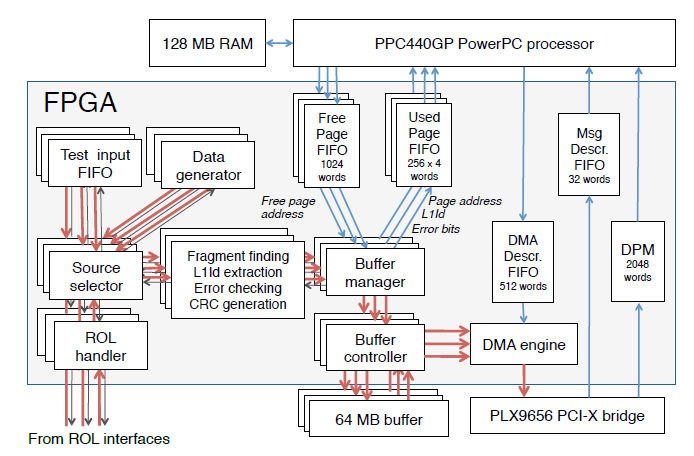
\includegraphics[scale=0.7]{whiteson2.png}
		\caption{Diagrama de bloques de la FPGA en ROBIN \cite{Whiteson2016TheSystem}.}
		\label{fig:whiteson2}
	\end{figure}
	
	\newpage
	Si bien este detector es comparativamente más complejo que los anteriores, presenta elementos comunes es su composición, sobretodo en la utilización de ASICs y FPGA para captura y control de los datos adquiridos. Se asemeja funcionalmente al PET 4D, en el sentido de implementar múltiples instancias de hardware equivalente, para así lograr manejar mayores cantidades de datos, brindando también mayor control e independencia en cada uno de ellos. El fuerte de este detector radica en su conectividad en red y sistemas distribuidos, necesarios para la gran cantidad de datos simultáneos que deben ser procesados. 

%\newpage
%\section{Síntesis}
%	Es claro que la tendencia es la utilización de ASICs en etapas de primera lectura y de FPGAs en etapas de manejo de datos y preprocesamiento, principalmente debido a la magnitud temporal de las señales, a la alta necesidad de precisión en su sincronización, y a la gran cantidad de señales de entrada que deben ser atendidas.
%	
%	Los elementos más utilizados y recomendados a implementar son los buffers de almacenamiento, principalmente para ajustar la tasa de transmisión de datos de la captura hacia las siguientes etapas de procesamiento, que suelen ser más lentas. En el sistema que se planea diseñar esto no es un problema, ya que la tasa de eventos es muy baja en comparación a los detectores estudiados. Aún así, pueden ser útiles para el escalamiento de los detectores en el futuro.
	
%	\par El concepto de serialización de datos estuvo principalmente presente en el detector LabPET II. Es pertinente considerarlo, sobretodo para el escalamiento del detector de muones. En caso de requerir cubrir un área mayor o con varias capas superpuestas de detectores, será necesario captar mayor cantidad de señales. Es allí donde se debe decidir si es recomendable comenzar con serialización de datos o con paralelismo de hardware. Además, dado que es necesario tener noción del tiempo de ocurrencia de los eventos, podría asociarse este dato a cada pulso, facilitando la implementación de serialización de datos. Esto no sería una desventaja, ya que no existe real necesidad de procesar datos de manera rápida y simultanea, reduciendo costos en hardware, pero aumentando esfuerzos de ingeniería.
%	
%	\par Para el caso de preprocesamiento, selección, formateo y transmisión de datos puede se considerar agregar procesadores dedicados en conjunto con la FPGA principal, que si bien no fueron encontrados textualmente en los ejemplos indicados, sí pueden ser de utilidad, sobretodo dada la existencias de chips que incluyen FPGA en conjunto con procesadores, como los SoC (\textit{System on Chip}) Zynq.
%	
%	\par Finalmente, puede ser interesante incluir métodos de TDC para conversión de la señal digital generada por la placa acondicionadora ASD. La duración de esta señal tiene relación con la amplitud y la energía de los pulsos analógicos captados, lo que podría ser muestreado con una implementación similar a la indicada en \cite{Arpin2010AResources}.
	